\documentclass{acm_proc_article-sp}

\usepackage[english]{babel}
\usepackage[utf8]{inputenc}
\usepackage{amsmath}
\usepackage{amssymb}
\usepackage{csvsimple}
\usepackage{framed}
\usepackage{graphicx}
\usepackage[colorlinks=true, pdfborder={0 0 0}, citecolor=blue, filecolor=blue, linkcolor=blue, urlcolor=blue]{hyperref}
\usepackage[colorinlistoftodos]{todonotes}
\usepackage{pgfplots}
\usepackage{pgfplotstable}

\title{Euler vs. Hamilton --- Investigating Claims of Quaternion Superiority for Rotation Parameterisation of Interactive 3D Camera Control Problems}
\author{}
\date{}

\begin{document}
\maketitle

\begin{abstract}
Precious little research exists on the optimal way to represent interactive cameras with three degrees of freedom.
These are cameras that can fly through a scene while rolling, pitching and yawing.
In addition, they are controlled by a user through use of the mouse and keyboard.
We investigate whether quaternions have the same numerical stability for this application area as for the integration case mentioned in \cite{zupan11}.
Along the way, we note several interesting phenomena we perceived during the course of our research.

In order to test this numerical stability, we compare the stability of our quaternion camera implementation against the implementation that has the best numerical stability that we know of --- the orthonormalised rotation matrix representation.
This representation has some advantages.
First, it is gimbal lock free (like quaternions), since there are no independent angles that can be rotated into one another's planes --- instead, the coordinate system as a whole rotates when the camera moves.
Second, it is a very intuitive system for graphics programmers who are already very familiar with rotation matrices.
Lastly, they are very stable numerically.

We also offer empirical evidence of the performance increase that can be obtained by using quaternions instead of rotation matrices.

\end{abstract}

\category{K.8.1}{Application Packages}{Graphics}

\terms{Algorithms, Experimentation, Measurement, Performance}

\section{Introduction}

Rotation --- or rather the \emph{representation} of rotation --- in three-dimensional affine space is surprisingly difficult.
There are many different ways to represent these rotations, e.g. Euler-angle, axis-angle, rotation matrices, or unit quaternion parameterisations.
Of these examples, the unit quaternion parameterisation is often said to be superior.
Quaternions solve the gimbal lock problems that Euler-angle systems experience, and are said to be more numerically stable.
It has also been claimed that quaternions are a more efficient method of calculating rotations.
We have no reason to doubt these claims, in fact they seem sensible to us and we present empirical evidence of their veracity.
However, we question the conclusion that all animation systems should use quaternions as a parameterisation of their rotations.
In this paper we will specifically look at the special case of an interactive three dimensional camera with three degrees of freedom (pitch, roll and yaw) in order to see whether the claims that quaternions are superior can be empirically supported.
These claims are that quaternions do not suffer from gimbal lock; are more numerically stable than other approaches; and more performant.
To the best of the authors' knowledge, there are no research papers that publish empirically derived figures supporting these claims.
It is important to have access to such figures, however, since what is true in theory may not hold up in practice once implemented on a real computer system ---
especially due to factors such as the numerical instability that is introduced by the inaccurate floating point mathematics as implemented for computers, or the fact that graphics cards and their drivers may have hidden performance cliffs and undocumented behaviour.
We have also been unable to find any discussion in the literature about which parameterisation to use for floating cameras with three degrees of freedom.
The contribution of this paper is then a conclusion as to this best possible parameterisation and the provision of empirical figures to back up various claims.

\section{Parameterisations}

Several parameterisations of rotations in three dimensions have already been proposed.
We recapitulate some of them here, for the uninitaited reader.

\subsection{Euler-Angle}

The Euler-angle system is a parameterisation based on three separate angles: roll, pitch and yaw --- these are the rotation amounts around three separate axes: the X, Y, and Z axes, respectively \cite{diebel06}.
The problem with this system is one of gimbal lock.
Briefly stated, a rotation of one of the axes can bring it into the plane of one of the other axes.
At this stage, a rotation about any one of these two axes is equivalent to a rotation about the other, leading to the loss of a degree of freedom \cite{pletinckx89}.

\subsection{Axis-Angle}

The axis-angle representation collapses all rotations to a rotation with a certain magnitude about a single axis.
The magnitude of this rotation becomes the length of a vector with a direction that corresponds to this axis \cite{diebel06}.

\subsection{Rotation Matrices}

Rotation matrices represent rotations as the components of a $3 \times 3$ matrix of real vlaues.
Rotation matrices are convenient because they work well with the well-established method of using matrices to represent affine transformations in computer graphics applications.
Rotation matrices have to be kept orthonormal, if they deviate from this property then they will alter the length of vectors, leading to distortions in the shape of the objects being rotated \cite{diebel06}.

\subsection{Quaternions}

Quaternion representations use a three component imaginary number vector along with a scalar component to represent rotations in three dimensional space.
They are convenient because composing rotations represented as quaternions is a simple matter of multiplying them together \cite{schoemake85}.
Other properties make quaternions more desirable than the other representations discussed so far.
For example, they are purportedly faster to compute than rotation matrices \cite{taylor79}, and they do not exhibit gimbal lock \cite{schoemake85}.

\section{Related Work}

The earliest mention of quaternions for use in representing rotations seem to be \cite{taylor79}, in which a novel method of robotic control is proposed.
Somewhat later \cite{schoemake85} proposed a rotation animation method that uses quaternions to interpolate between key frames.
That work claims that quaternions are best for interpolation \cite{schoemake85}.
Pletinckx in 1989 describes quaternions and makes the important point that they are a less redundant representation of rotation than rotation matrices, since they only have four components and not nine \cite{pletinckx89}.
The rest of that work motivates the use of quaternions in general graphics applications for such reasons as the fact that they are gimbal lock free \cite{pletinckx89} and can be used to solve animation, modelling and rendering problems \cite{pletinckx89}.
Mukundan's work is a similar paper on the desirability of quaternions, pointing to applications in computer vision \cite{mukundan02}.
Zupan presents a recent paper that describes a method for integrating rotation values from angular velocity through the use of quaternions \cite{zupan11}.
In that paper, it was discovered that quaternion representations offer the least amount of numerical instability for this application area.
The rest of this paper will attempt to replicate this numerical stability in the realm of interactive camera control, and also comment on various phenomena found along the way.

\section{Experimental Setup}

Our experiment consists of an implementation of both competing methods of interactive camera control.
The first implementation stores the current camera's orientation as a rotation matrix.
This rotation matrix is then multiplied by rotation matrices that indicate the amount to rotate by whenever the camera's orientation is altered.
The second implementation stores the current camera's orientation as a quaternion.
The quaternion is then multiplied by another quaternion that indicates the adjustment in the camera's orientation whenever the mouse is moved.
We implement these camera algorithms as C++ templates and instantiate them with both single and double precision floating point types.
Each implementation is also accompanied by a version that orthonormalises the rotation sub-matrix before it is sent to the shaders to be used as a view matrix.

\begin{figure}
\begin{framed}
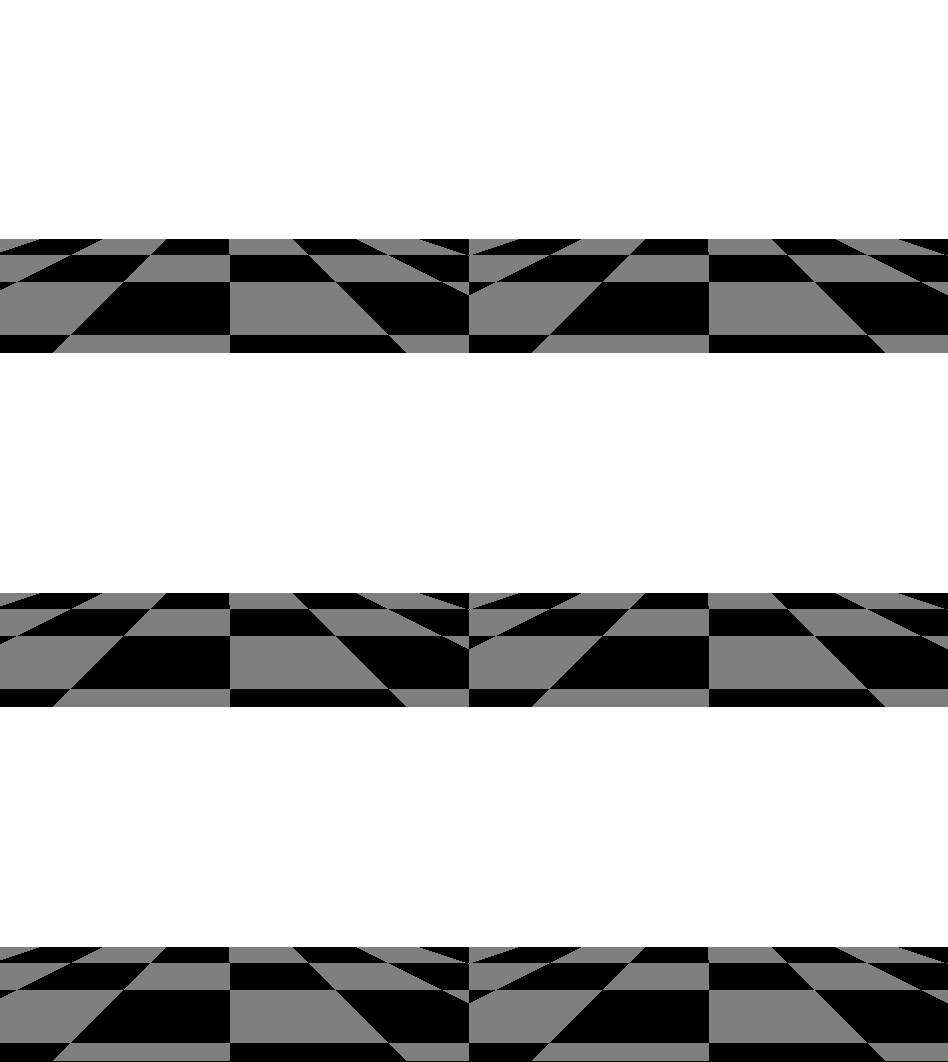
\includegraphics[width=8cm]{user_interface.png}
\caption{The user interface for the test platform.}
\end{framed}
\end{figure}

The user is now presented with a simple scene that contains some basic geometry to allow the user to orient him / herself.
By moving the mouse, the user can rotate the camera about its X or Y axes.
Keyboard controls allow the user to move the camera forward, back and to the left and right.
The keyboard also allows the user to ``roll'' the camera around the Z axis.

The algorithms we tested are the normal rotation matrix implementation, the orthonormalised matrix implementation, the quaternion implementation, and an orthonormalised quaternion implementation.
We tested an orthnormalised quaternion implementation as well, since the quaternion implementation was so much cheaper, it is fair to allow it to spend more time to obtain the same accuracy as the other methods.
Unfortunately, this did not work out.
The orthonormalisation technique that was used is the Gram-Schmidt method.

With each alteration of the camera's position or orientation we obtain the resulting view matrix for each algorithm's single precision and double precision versions.
For each element of the view matrix, we subtract the single precision value from the double precision value.
We assume that the latter will be more accurate than the former.
Therefore, this subtraction indicates the amount of error in the single precision value.
We average the result of each of these subtractions to obtain an overall error value for that algorithm.

Next, the algorithms are compared against one another for each mouse / keyboard movement.
If an algorithm has an error value that is less than that of its competitors, it is awarded a win.
At the end of the test run, the algorithm with the most wins is deemed the most numerically stable.

Thirty tests of that were approximately one minute in length each were run, recording the victorious algorithm after each test has terminated.

\section{Results} 

We have reproduced some graphs detailing the numerical stability of the various algorithms over time for several of our experimental test runs in Figure \ref{fig:stability}.

Performance graphs can be found in Figure \ref{fig:performance}.

\begin{figure}[htpb]
\begin{framed}
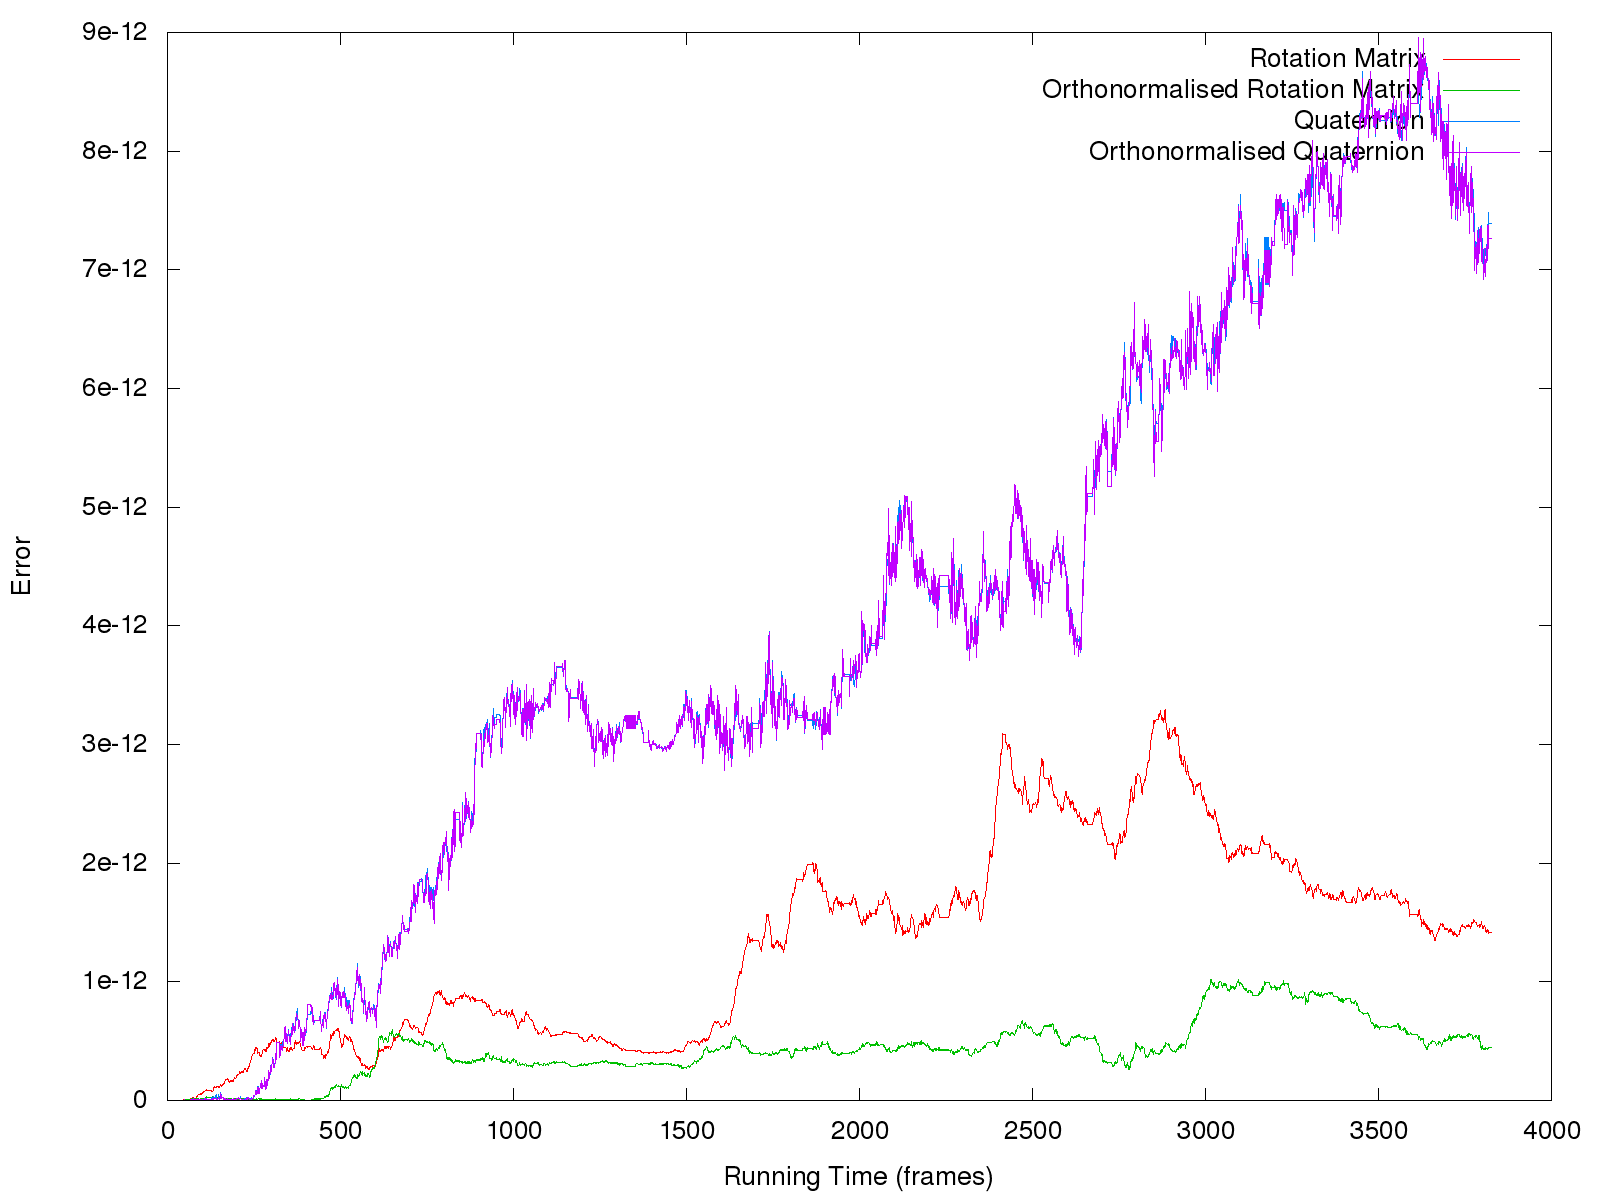
\includegraphics[width=8cm]{plots/stability_plot_21.png}
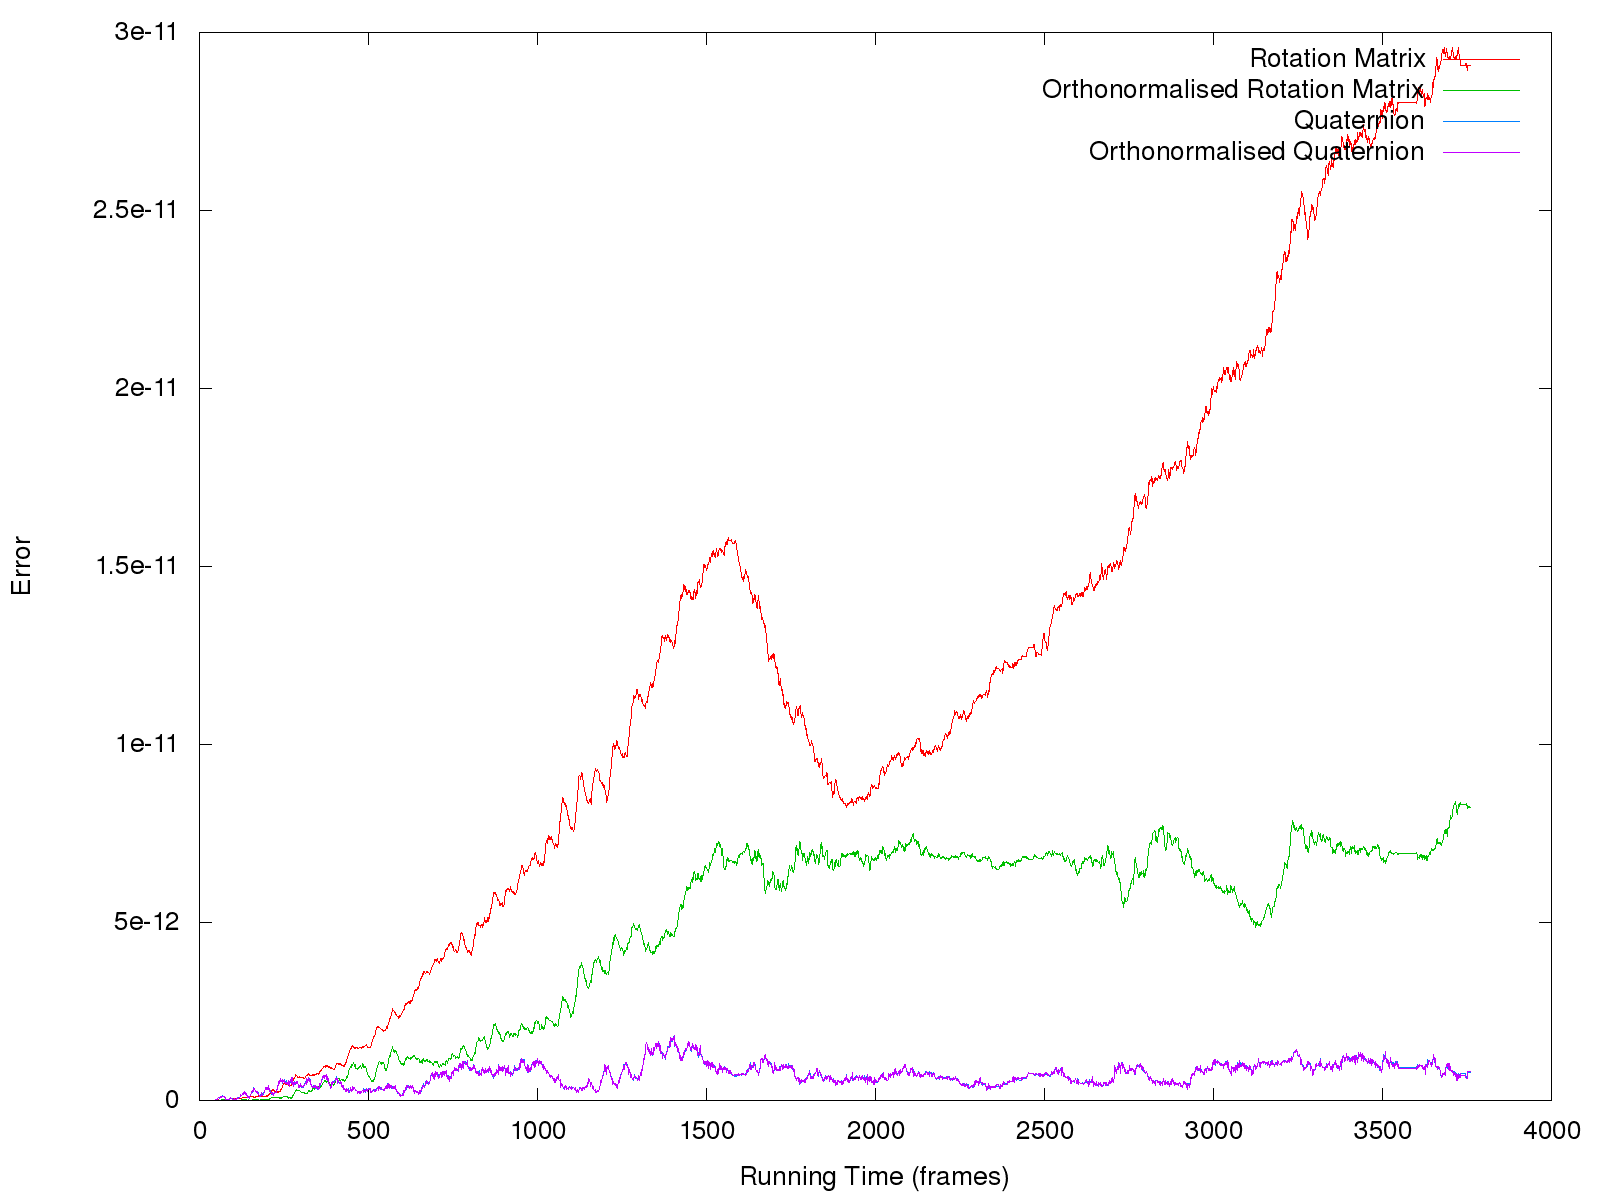
\includegraphics[width=8cm]{plots/stability_plot_13.png}
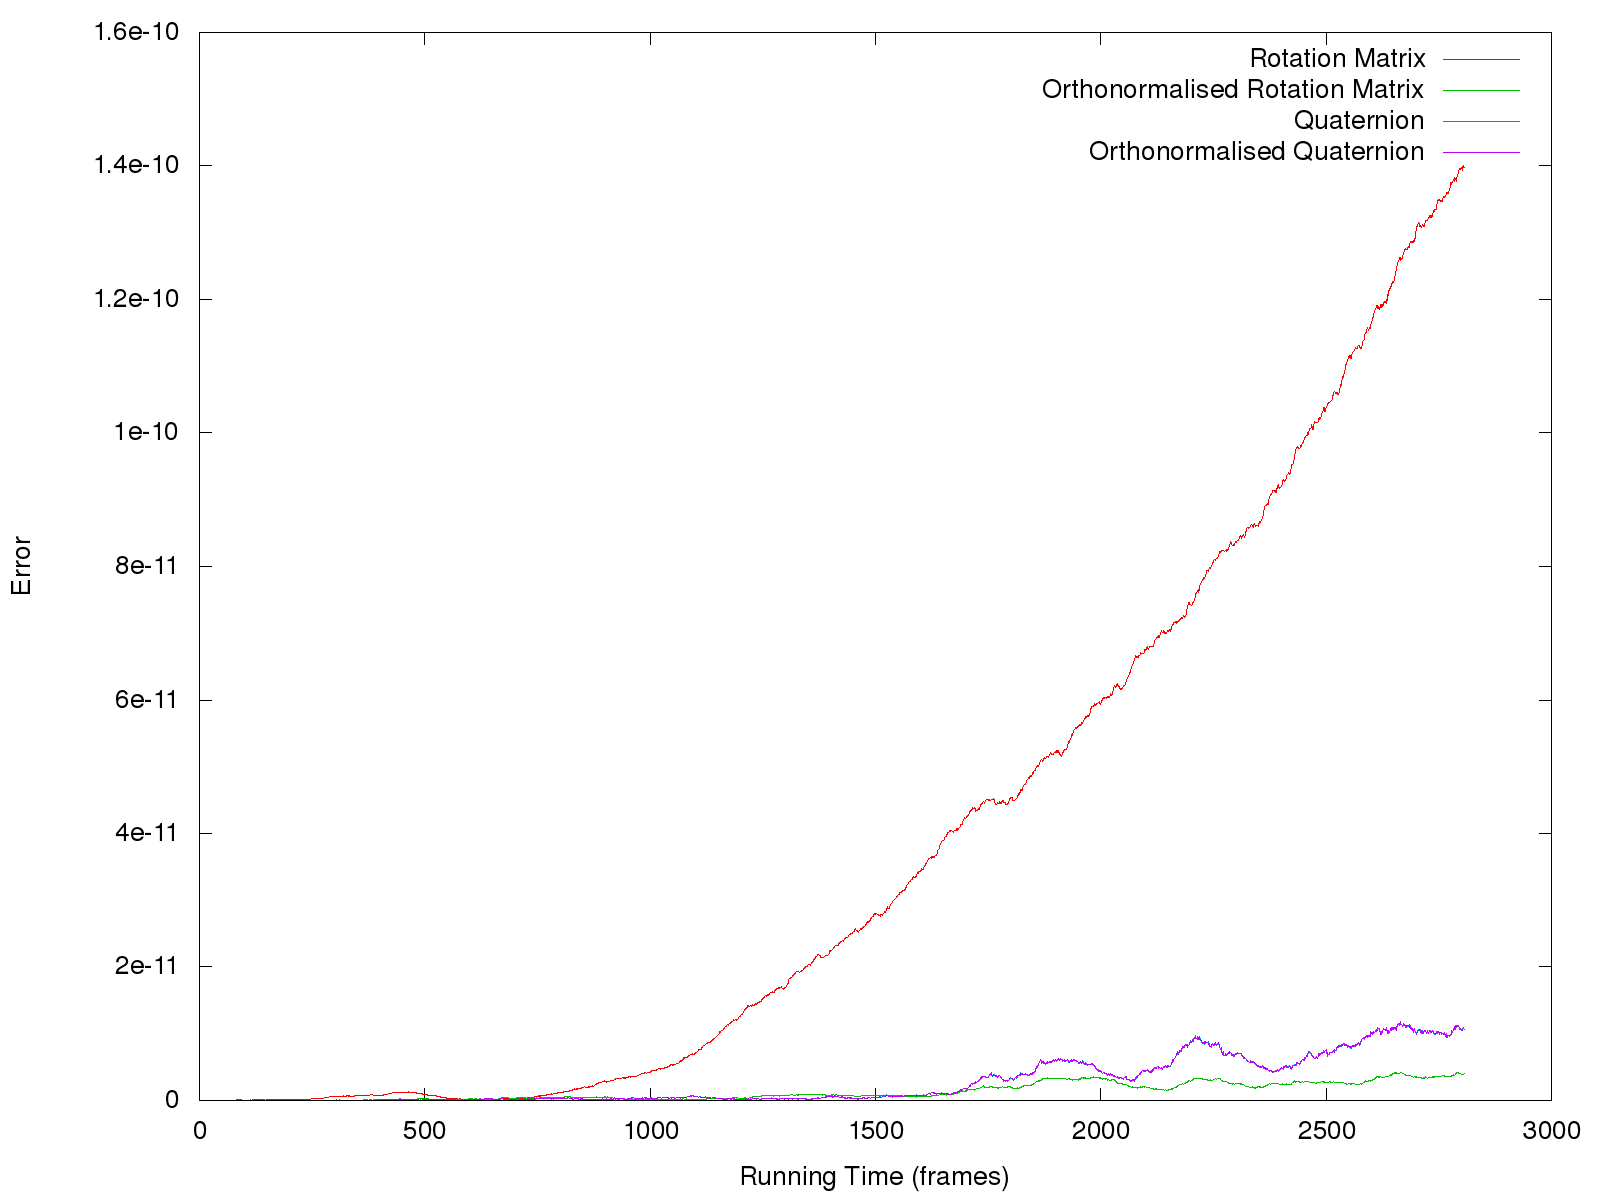
\includegraphics[width=8cm]{plots/stability_plot_28.png}
\caption{In these graphs, the X axis indicates time, and the Y axis indicates the total accumulated error value.
Test run 21 (top) indicates a case where quaternions performed relatively poorly in terms of numerical stability.
Test run 13 (middle) illustrates a rare case where the orthonormalised rotation matrix performance was sub par.
Test run 28 (bottom) illustrates the poor stability of rotation matrices without orthonormalisation.}
\label{fig:stability}
\end{framed}
\end{figure}

\begin{figure}[htpb]
\begin{framed}
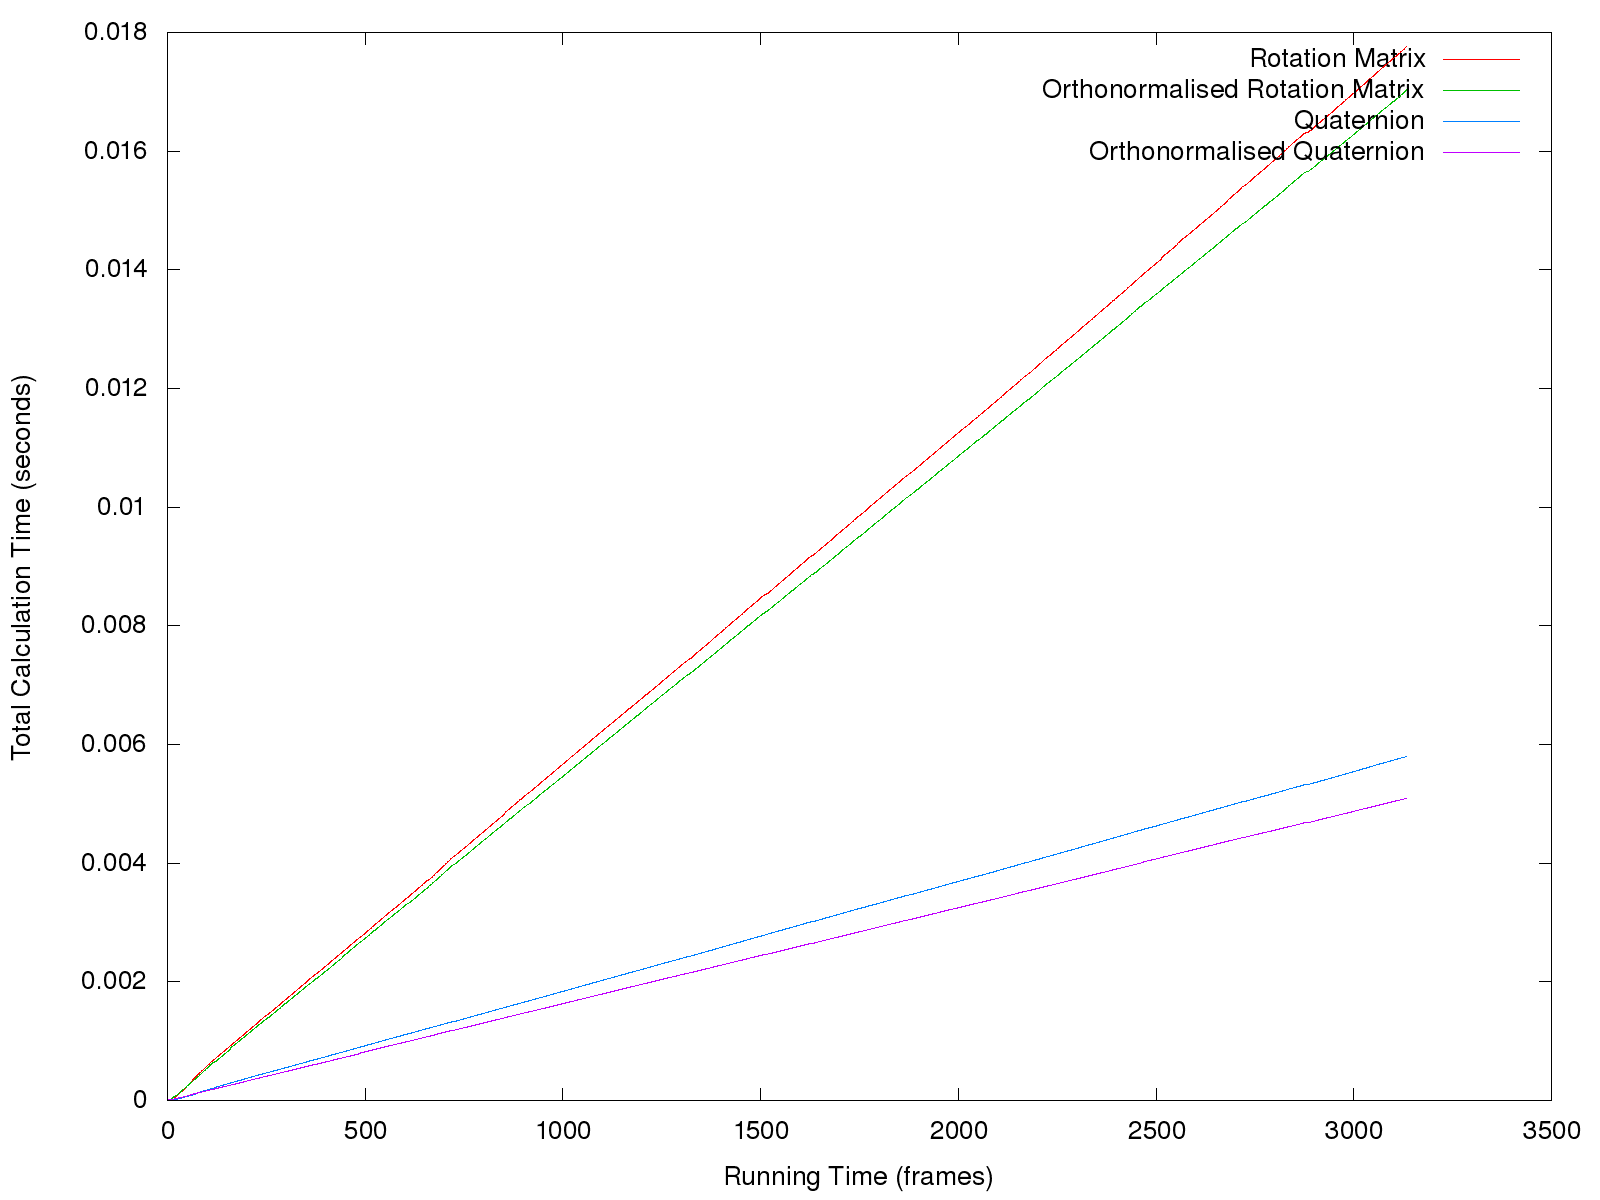
\includegraphics[width=8cm]{plots/timing_plot_1.png}
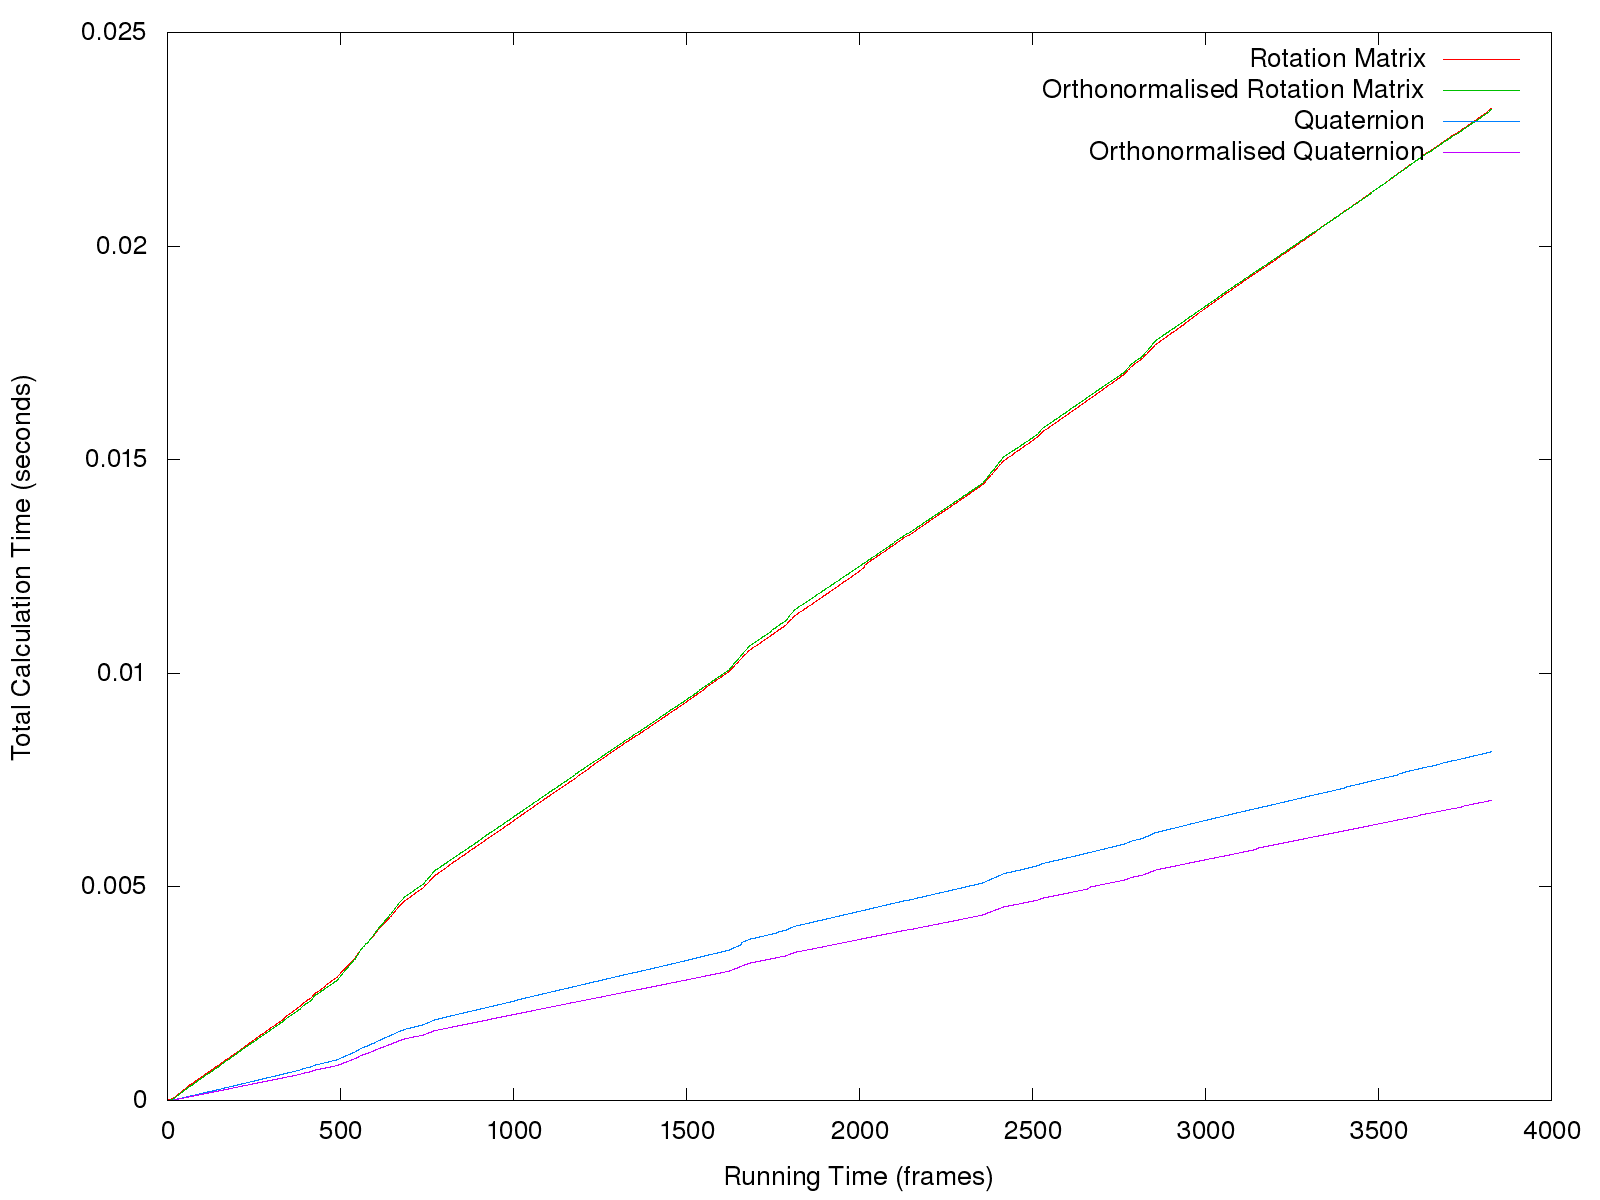
\includegraphics[width=8cm]{plots/timing_plot_21.png}
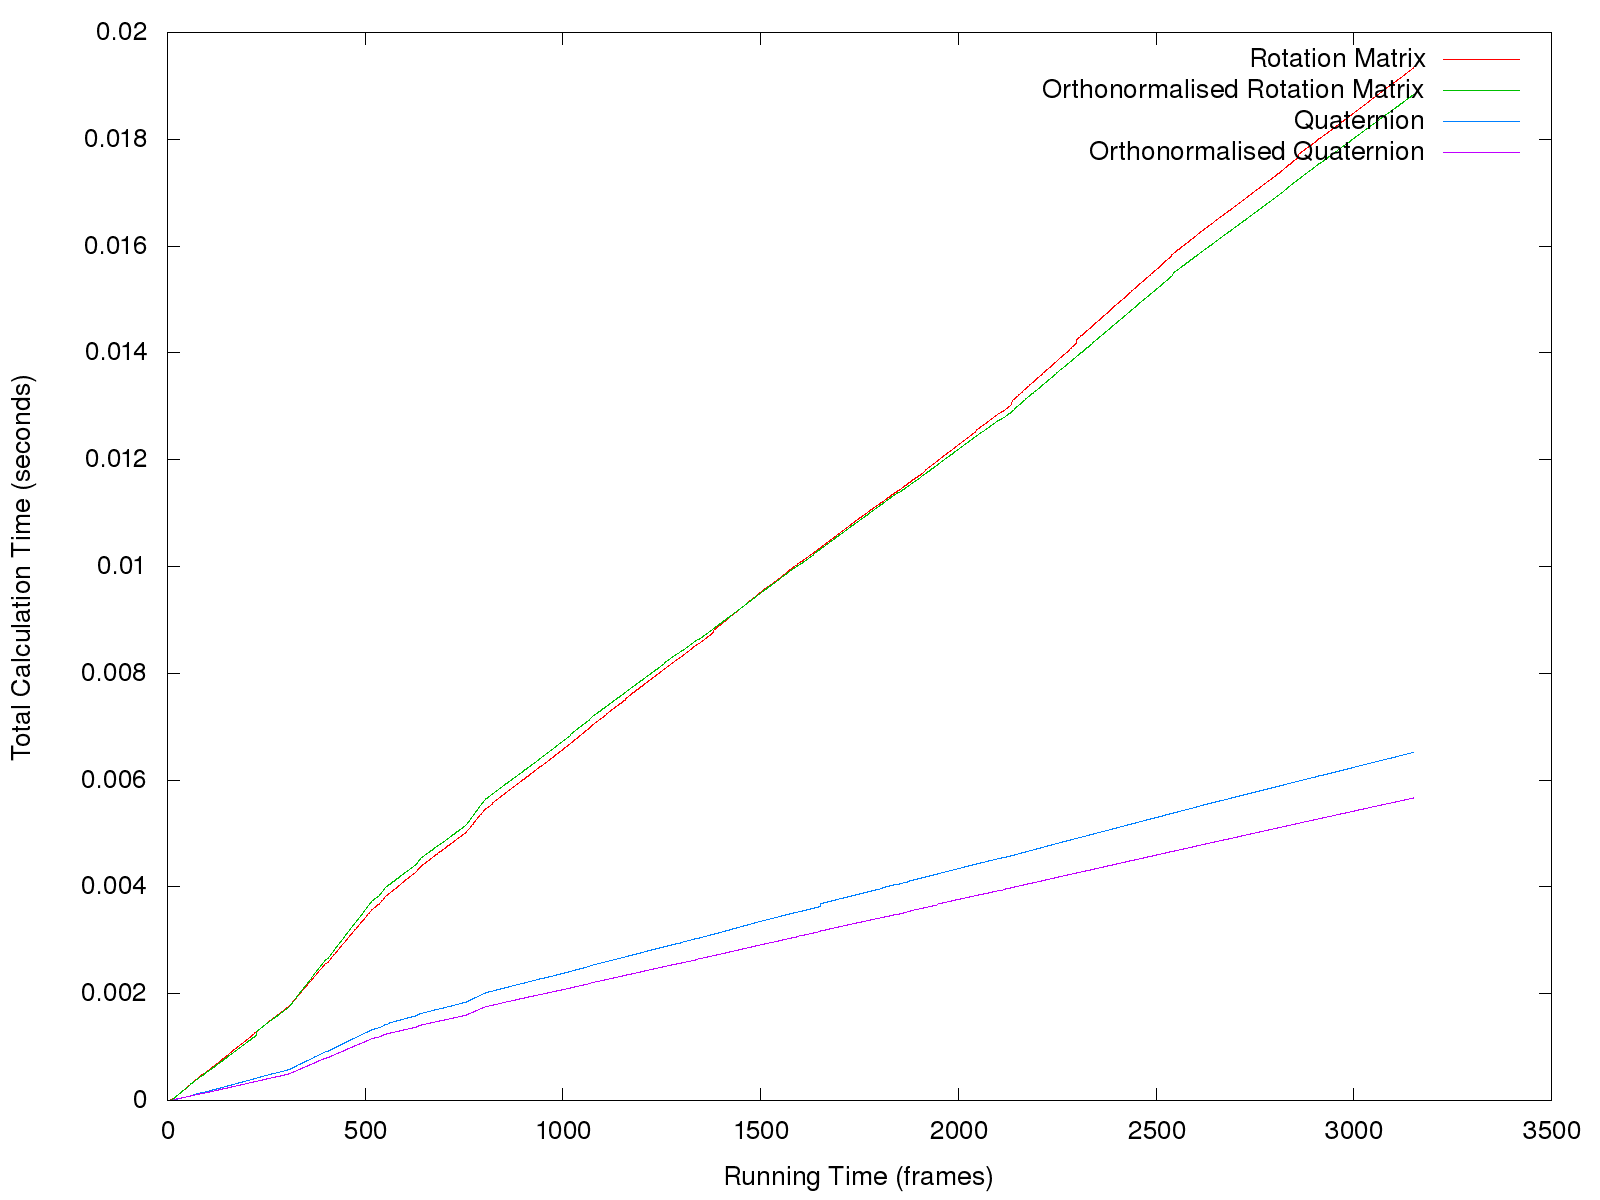
\includegraphics[width=8cm]{plots/timing_plot_22.png}
\caption{In these graphs, the X axis indicates time, and the Y axis indicates the total time spent calculating view matrices by each algorithm.
Test run 1 (top) is a typical performance profile.
Test run 21 (middle) is curios, the orthonormalisation does not seem to cost anything for the rotation matrix.
Test run 22 (bottom) is more anomolous, note that the orthonormalised rotation matrix is less expensive than the non-normalised version.}
\label{fig:performance}
\end{framed}
\end{figure}

In general, it was found that the orthonormalised rotation matrix performed the best in terms of numerical stability.
This is discussed in subsection \ref{sec:stability}.

The orthonormalisation of the quaternion representation's resulting view matrix had almost no effect on the numerical stability of that algorithm.
Why this should be the case is an excercise for future work.

An interesting result is that the quaternion algorithms are actually faster than the rotation matrix versions.
This is in line with the passing comment made by Taylor \cite{taylor79}.
This phenomenon is described in subsection \ref{sec:performance}.

\subsection{Numerical Stability}
\label{sec:stability}

The results of our numerical stability experiment is represented in the table below.

\begin{figure}
\csvautotabular{wins.csv}
\caption{Table of wins for an algorithm per test run.}
\label{fig:wins}
\end{figure}

In Figure \ref{fig:wins}, ``RotMat'' represents the na\"{i}ve rotation matrix implementation. ``OrthoRotMat'' is the rotation matrix implementation that uses orthonormalisation, ``Quat'' is the quaternion implementation, and ``OrthoQuat'' is the quaternion implementation that uses orthnormalisation.

It is an exception when the orthonormalised implementation is not superior for most of the run of an experiment.
In fact, ``OrthoRotMat'' only loses out in two out of thirty cases.

The odds of obtaining this result at random (assuming the null hypothesis that all algorithms are equally stable) is $\left(\dfrac{1}{4}\right)^{28} \approx 1.39e^{-17}$.
We therefore regard this result as significant.

We typically observed that the orthnormalised rotation matrix and quaternion implementations remained at an error level around the $10^{-12}$ level, 
The na\"{i}ve rotation matrix quickly exploded to the $10^{-10}$ level or even exceeded it.

\subsection{Relative Performance}
\label{sec:performance}

One might expect that quaternions are somewhat slower than rotation matrices, since they need to be converted to a new format, and because the math describing them is somewhat complex.
This turns out not to be the case, as the table in Figure \ref{fig:performance-table} will show (printed in Appendix A, due to formatting issues).

Two things are interesting from this table.
First, the quaternion implementations are faster than the rotation matrix implementations.
This is proof of Taylor's aside to that effect in his paper \cite{taylor79}, and Schoemake's affirmation of that statement \cite{schoemake85} --- quaternions are indeed much faster than rotation matrices.
In fact, the speed increase is approximately an order of magnitude.

Second, the orthonormalised version of the algorithms are often cheaper than the non-normalised version.
The reason for this is left as an excercise for future research.

Returning to the question of the relative performanc of quaternions to rotation matrices, we could not find a discussion on why this should be so from a mathematical point of view.
We have therefore performed such an analysis below.

Consider a case where a view matrix representation has to be updated with a rotation around two axes, for example the X and Y axes.
(We ommit the Z axis from this consideration, because it is implemented in exactly the same way as the X and Y axes, and therefore doesn't affect a comparison between methods if it is left out.)
The current rotation matrix is a four dimensional matrix in homogenous coordinate space, and so is the rotation matrix for the X and Y axes.
The current rotation matrix is given by:

$R = \left[ \begin{array}{cccc}
    R_{11} & R_{12} & R_{13} & R_{14} \\
    R_{21} & R_{22} & R_{23} & R_{24} \\
    R_{31} & R_{32} & R_{33} & R_{34} \\
    R_{41} & R_{42} & R_{43} & R_{44} \\
\end{array} \right]$

Then the X and Y update matrices are given by:

\vspace{0.5em}
$X = \left[ \begin{array}{cccc}
    X_{11} & X_{12} & X_{13} & X_{14} \\
    X_{21} & X_{22} & X_{23} & X_{24} \\
    X_{31} & X_{32} & X_{33} & X_{34} \\
    X_{41} & X_{42} & X_{43} & X_{44} \\
\end{array} \right]$, and

$Y = \left[ \begin{array}{cccc}
    Y_{11} & Y_{12} & Y_{13} & Y_{14} \\
    Y_{21} & Y_{22} & Y_{23} & Y_{24} \\
    Y_{31} & Y_{32} & Y_{33} & Y_{34} \\
    Y_{41} & Y_{42} & Y_{43} & Y_{44} \\
\end{array} \right]$

The update step then involves an equation like $R\prime = RXY$ where $R\prime$ is the new rotation matrix.
This involves two $4 \times 4$ matrix-matrix multiplications, which can be decomposed into two sets of dot products between the columns and rows of each matrix.
Since each matrix is $4 \times 4$, this is approximately 32 dot products in total.
Each dot product contains 3 summation operations and 4 multiplies, which leads to a total of 96 summations and 128 multiplies for the matrix-matrix multiplication alone.
In addition, a further four transcendental function invocations each are required to calculate X and Y.
Finally, the Gram-Schmidt orthonormalisation process is applied, but since we applied this to the quaternion implementation as well, it is not necessary to count its operations.

For the quaternion implementation, matters are different.
First, the quaternion rotations about the X and Y axes must be converted from an angle-axis representation.
This involves 2 transcendental function invocations as well as 5 multiplications for both the X and the Y quaternion, for a total of 4 transcendental function invocations and 10 multiplications \footnote{\url{https://github.com/g-truc/glm/blob/0.9.5/glm/gtc/quaternion.inl} (Last Accessed 2014-06-23.)}.
Next the quaternions must be multiplied.

Consider two quaternions: $q_1$ and $q_2$.
Now, each quaternion consists of one real part (which we can treat as a scalar) and an imaginary part (which we treat as a three-component vector).
Label these scalars and vectors as $s_1$, $s_2$, $v_1$, $v_2$, respectively.
If we rewrite $q_1$ as $\left[ \begin{array}{cc} s_1 & v_1 \end{array} \right]$ and $q_2$ as $\left[ \begin{array}{cc} s_2 & v_2 \end{array} \right]$ then quaternion multiplication is simply defined as $q_1 q_2 = \left[ \begin{array}{cc} s_1 s_2 - v_1 \cdot v_2 & s_1 v_2 + s_2 v_1 + v_1 \times v_2 \end{array} \right]$ \cite{schoemake85}.
This calculation involves 3 scalar multiplications, 1 addition, 1 subtraction, a dot product and a cross product.
The dot product consists of 3 multiplies and 2 adds.
The cross product comprises 6 multiplies and 3 subtractions.
This brings the subtotal for a single quaternion multiplication to 12 multiplies, 3 additions, and 3 subtractions.
Since two multiplications are necessary, that brings the subtotal for quaternion multiplications to 24 multiplies, 6 additions and 6 subtractions.

The final step in the quaternion algorithm is to translate the quaternion into a rotation matrix.
If a quaternion can be written as $q = \left[ \begin{array}{cccc} w & x & y & z \end{array} \right]$, where $w$ is the scalar part from before, and $\left[ \begin{array}{ccc} x & y & z \end{array} \right]$ are the components of the imaginary part discussed earlier, then this translation is given by the matrix $M$ where

$M = \left[ \begin{array}{ccc}
    1 - 2y^2 - 2z^2 & 2xy + 2wz & 2xz - wy \\
    2xy - 2wz & 1 - 2x^2 - 2z^2 & 2yz + 2wz \\
    2xz + 2wy & 2yz - 2wx & 1 - 2x^2 - 2y^2 \\
    \end{array}\right]$

This operation involves 36 multiplies, 3 additions and 9 subtractions.
However, this operation only needs to be performed once, since it is only the resulting quaternion that needs to be converted to a matrix for use as the view matrix by the shader programs.
The results of this instruction counting exercise are summarized in Figure \ref{fig:counting}.

Nearly every category of instruction is much larger for the rotation matrix parameterisation than for the quaternion version.
Therefore, it should not be surprising that the quaternion implementation is so much faster.

\begin{figure}
\begin{framed}
\begin{tabular}{l|l|l|l|l}
    Algorithm       & $\sin$/$\cos$  & $\times$      & $+$       & $-$  \\
    \hline
    Rotation Matrix & 8              & 128           & 96        & 0             \\
    Quaternion      & 4              & 70            & 9         & 15            \\

\end{tabular}
\caption{Instruction counting for rotation matrix and quaternion algorithms.}
\label{fig:counting}
\end{framed}
\end{figure}

\section{Conclusion}

We have empirically verified various claims about unit quaternions and their use as rotation parameterisations.
They are somewhat faster than rotation matrices.
The difference is about a two to three times speed increase, but the absolute values are already so low that it is likely that this difference will only matter in heavily resource-constrained environments.

In addition, the numerical stability that quaternion rotation parameterisations enjoy in the integration of rotational velocities does not extend to interactive camera control environments.
In these environments, the orthonormalised rotation matrix is superior in the realm of numerical stability.
The difference is negligable, however, and the quaternion implementation is somewhat faster.
We suspect that this difference will only matter in situations where numerical stability is \emph{very} important, such as extremely sensitive robot control problems or very long running processes that can accumulate large amounts of errors.

Finally, we have discovered that the Gram-Schmidt orthonormalisation that was used in this experiment has almost no cost associated with it, and indeed, sometimes saves computational time.
The reason for this is likely related to compiler or central processing unit optimizations, but we leave further speculation on that front to future work.

\section{Additional Materials}

The full source code repository, as well as all collected data, will be released should the paper be accepted.
For now, it has been removed to protect the anonymity of the researchers.

\bibliographystyle{ACM-Reference-Format-Journals}
\bibliography{main}

\onecolumn
\newpage

\section*{Appendix A}

\begin{figure}[h]
\csvautotabular{performance.csv}
\caption{Time taken to calculate the camera's view matrix for each algorithm during each test run.
The times were produced by taking the total amount of time each algorithm spent on calculations, and dividing it by the total amount of times the mouse was moved.
Times are in milliseconds.}
\label{fig:performance-table}
\end{figure}

\end{document}
